% Graphic for TeX using PGF
% Title: /home/FatLord/Diagrama5.dia
% Creator: Dia v0.97.3
% CreationDate: Wed Oct  7 22:17:12 2015
% For: FatLord
% \usepackage{tikz}
% The following commands are not supported in PSTricks at present
% We define them conditionally, so when they are implemented,
% this pgf file will use them.
\ifx\du\undefined
  \newlength{\du}
\fi
\setlength{\du}{15\unitlength}
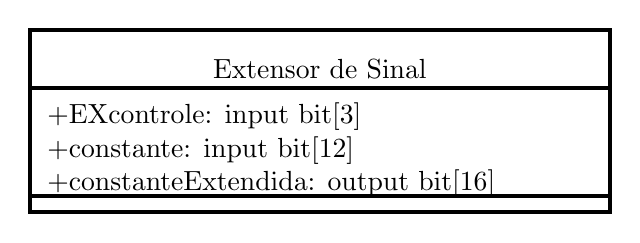
\begin{tikzpicture}
\pgftransformxscale{1.000000}
\pgftransformyscale{-1.000000}
\definecolor{dialinecolor}{rgb}{0.000000, 0.000000, 0.000000}
\pgfsetstrokecolor{dialinecolor}
\definecolor{dialinecolor}{rgb}{1.000000, 1.000000, 1.000000}
\pgfsetfillcolor{dialinecolor}
\pgfsetlinewidth{0.100000\du}
\pgfsetdash{}{0pt}
\definecolor{dialinecolor}{rgb}{1.000000, 1.000000, 1.000000}
\pgfsetfillcolor{dialinecolor}
\fill (14.700000\du,10.750000\du)--(14.700000\du,12.150000\du)--(28.675000\du,12.150000\du)--(28.675000\du,10.750000\du)--cycle;
\definecolor{dialinecolor}{rgb}{0.000000, 0.000000, 0.000000}
\pgfsetstrokecolor{dialinecolor}
\draw (14.700000\du,10.750000\du)--(14.700000\du,12.150000\du)--(28.675000\du,12.150000\du)--(28.675000\du,10.750000\du)--cycle;
% setfont left to latex
\definecolor{dialinecolor}{rgb}{0.000000, 0.000000, 0.000000}
\pgfsetstrokecolor{dialinecolor}
\node at (21.687500\du,11.700000\du){Extensor de Sinal};
\definecolor{dialinecolor}{rgb}{1.000000, 1.000000, 1.000000}
\pgfsetfillcolor{dialinecolor}
\fill (14.700000\du,12.150000\du)--(14.700000\du,14.750000\du)--(28.675000\du,14.750000\du)--(28.675000\du,12.150000\du)--cycle;
\definecolor{dialinecolor}{rgb}{0.000000, 0.000000, 0.000000}
\pgfsetstrokecolor{dialinecolor}
\draw (14.700000\du,12.150000\du)--(14.700000\du,14.750000\du)--(28.675000\du,14.750000\du)--(28.675000\du,12.150000\du)--cycle;
% setfont left to latex
\definecolor{dialinecolor}{rgb}{0.000000, 0.000000, 0.000000}
\pgfsetstrokecolor{dialinecolor}
\node[anchor=west] at (14.850000\du,12.850000\du){+EXcontrole: input bit\ensuremath{[}3\ensuremath{]}};
% setfont left to latex
\definecolor{dialinecolor}{rgb}{0.000000, 0.000000, 0.000000}
\pgfsetstrokecolor{dialinecolor}
\node[anchor=west] at (14.850000\du,13.650000\du){+constante: input bit\ensuremath{[}12\ensuremath{]}};
% setfont left to latex
\definecolor{dialinecolor}{rgb}{0.000000, 0.000000, 0.000000}
\pgfsetstrokecolor{dialinecolor}
\node[anchor=west] at (14.850000\du,14.450000\du){+constanteExtendida: output bit\ensuremath{[}16\ensuremath{]}};
\definecolor{dialinecolor}{rgb}{1.000000, 1.000000, 1.000000}
\pgfsetfillcolor{dialinecolor}
\fill (14.700000\du,14.750000\du)--(14.700000\du,15.150000\du)--(28.675000\du,15.150000\du)--(28.675000\du,14.750000\du)--cycle;
\definecolor{dialinecolor}{rgb}{0.000000, 0.000000, 0.000000}
\pgfsetstrokecolor{dialinecolor}
\draw (14.700000\du,14.750000\du)--(14.700000\du,15.150000\du)--(28.675000\du,15.150000\du)--(28.675000\du,14.750000\du)--cycle;
\end{tikzpicture}
